\chapter{Existing tracklet building solutions}\label{chap:existing_solutions}

\section{k-d trees}\label{sec:kd_trees}
	
	k-dimensional trees (k-d trees) are a hierarchical data structure that recursively partitions both the set of data points and the space in which they reside into smaller subsets and subspaces. Each node in a k-d tree represents a partial region of the whole space and a set of points contained in the region \citep{Bentley:1975:MBS:361002.361007}.
	
	Complexity of k-d trees is similar, or identical in some cases, to other tree data structures. For example, adding a point into a balanced k-d tree takes $O(log\ n)$ time and removing a point from a balanced k-d tree takes $O(log\ n)$ time as well. There are several approaches to constructing a k-d tree, such as finding a median among points (with complexity $O(n)$), sorting all points (with complexity $O(log\ n)$) or sorting a fixed number of randomly selected points.

\subsection{Efficient intra- and inter-night linking of asteroid detections using kd-trees}\label{subsec:intra_inter}

	The main focus of the paper (see \citep{kubica}) is the description of then under development Panoramic Survey Telescope and Rapid Response System (Pan-STARRS). The paper describes the capabilities of the system in areas such as identification of detection of moving objects in our solar system and linking of those detections within and between nights, attributing those detections to catalogued objects, calculating initial and differentially corrected orbits and orbit identification. Further, it illustrates k-d tree algorithms as suitable for linking of objects. The paper contains the description of their own pseudo-realistic simulation of the Pan-STARRS survey strategy and shows the results on both simulated and real data sets.
	
\subsubsection{Pan-STARRS}
	
	The paper describes future goals of Pan-STARRS - obtaining two images per night of each Solar System survey field and using these images to distinguish between real and false detections and to separate stationary and moving transient near-Earth objects (NEOs). The object is obtained and verified across several consecutive nights in order to have high probability of being real and to be able to be submitted to the Minor Planet Center (MPC, see Chapter \ref{chap:results}, Section \ref{sec:mpc})
	
\subsubsection{Pan-STARRS MOPS}
	
	Images are firstly preprocessed - cosmic rays and other noise or irrelevant objects need to be removed, they are aligned and combined into a single image. The resulting image is called \emph{master image} in the paper and is further combined with other master images to create a static-sky image used to produce yet another image containing only transient sources and noise. It is then searched for asteroids and comets. The preprocessing phase ends with all the identified sources from both images, along with their metadata (time, trail length, axis orientation, flux, etc.), being passed to the later stages.
	
	The first step - linking intra-night detections of spatially and temporally close objects, which, in addition, have fixed speed among multiple detections, into tracklets - is being done by comparing expected and detected trail length and orientation. Only the objects which pass through this filter are combined into tracklets. The second step is the inter-night linking of tracklets into collections called tracks. The tracks are verified by IOD (see Chapter \ref{chap:object_dynamics}, Section \ref{sec:init_orbit_det}) and Orbit Determination (OD, see \citep{klinkrad2006space}). The complexity of the linking increases like $\rho^2$, where $\rho$ is the number of detections/deg$^2$. This can be solved by employing k-d trees to reduce the complexity that increases like $\rho\ log\ \rho$ \citep{kubica}.
	
	\begin{figure}[H]
	\centering
	  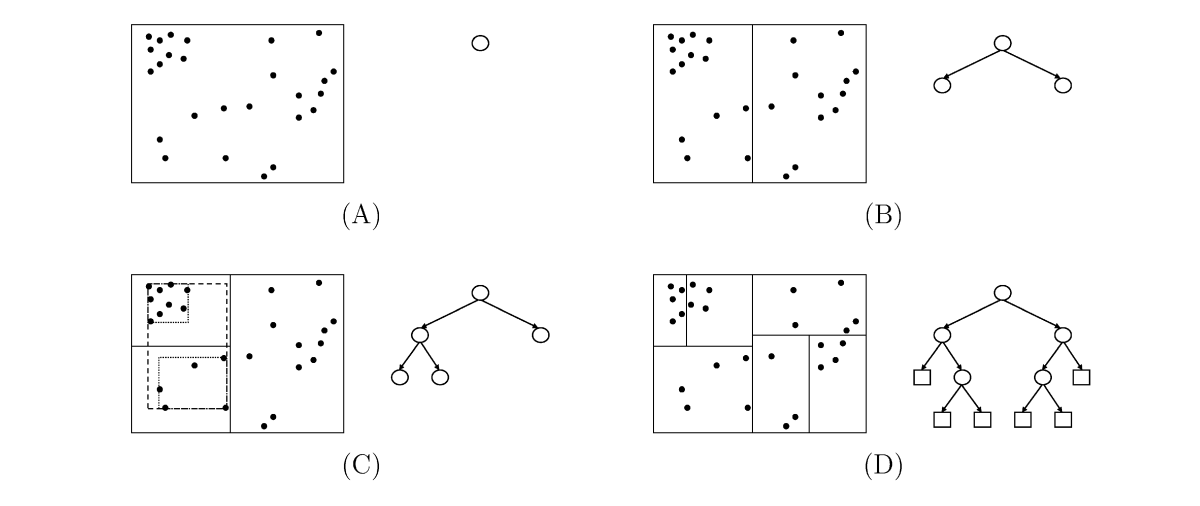
\includegraphics[width=10cm]{images/kd_tree}
		  \caption{k-d tree schematic. Image from \citep{kubica}.}
	  \label{fig:kd_tree}
	\end{figure}
	
	The k-d tree is created from top to bottom, having full image as the root node. At each level the data in form of points is used to create a bounding box which is then saved in the corresponding node. The points are then split into two disjoint sets at the widest dimension of the node and bounding boxes are created and assigned again. The recursion is stopped when the currently created node owns less than pre-determined number of points and such node is marked as a leaf node. The construction process is illustrated in Figure \ref{fig:kd_tree}.
	
	Searching for spatially close nodes is done by descending the tree depth first and searching for points within a radius. If the algorithm finds a node that falls out of the radius it stops because it is guaranteed that each child of the node will fall out of the radius as well. If the algorithm reaches a leaf node, the points in it are tested for the distance from the point of query and eventually added to the results. The algorithm is extended by another constraint - temporal significance. In the paper, they consider each detection as the start of a potential tracklet and look at temporally subsequent detections to judge their relevance and add them to the tracklet. Time is added to the k-d tree as a third dimension. The result of having time as the third dimension is illustrated in Figure \ref{fig:kd_tree_time} as a cone which spread is controlled by the maximum allowed speed.
	
	\begin{figure}[H]
	\centering
	  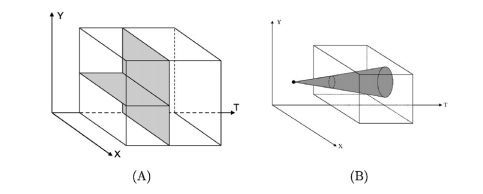
\includegraphics[width=10cm]{images/kd_tree_time}
		  \caption{k-d tree temporal search. Image from \citep{kubica}.}
	  \label{fig:kd_tree_time}
	\end{figure}
	
	Inter-night linking is out of scope of this thesis, similarly to creation of synthetic data and their description can be found in the paper - see \citep{kubica}.

\section{Uniform linear motion detection}\label{sec:linear_motion}
	
	Linear motion is a one dimensional motion along a straight line and mathematically can be explained using one spatial dimension. One of the two types of linear motion is uniform linear motion, which has constant velocity. In the most cases space debris does not follow straight line nor its acceleration is zero. However, when observing under narrow enough field of view (FOV), only part of its trajectory is captured and the object moves according to uniform linear motion.

\subsection{Optical observation, image-processing, and detection of space debris in GEO}\label{subsec:linear_geo}

	The paper (see \citep{oda}) describes an efficient detection of space debris on GEO orbit using a telescope with 3.17° FOV producing images with a resolution of $2048 x 2048$. The authors describe image processing and the successive application of the uniform linear motion algorithm to detect objects which are then either matched with the USSTRATCOM catalogue or classified as newly discovered debris.
	
\subsubsection{Image processing}

	The image is preprocessed by subtracting a master dark bias frame from raw images to reduce noise, correcting the sensitivity of pixels and uneven illumination, masking bright pixels and subtracting the sky background frame. Due to the long exposure of 4.7 sec, the stars appear as streaks approximately 13 pixels long and are removed. Noise, such as cosmic rays, do not have diffusive shape and are removed too. The resulting image contains objects that have diffusive shape and are extracted by Gaussian fitting \citep{oda}.
	
\subsubsection{Detection algorithm}

	The detection algorithm is based on the facts mentioned in Section \ref{sec:linear_motion} - when we select small enough part of the whole trajectory of an object, the part adheres to the uniform linear motion. After selecting an appropriate candidate from an image (an object having sufficient intensity and correct shape), the next image is considered and only objects that show uniform linear motion and are the brightest are picked. This procedure is repeated until there are 9 positive matches out of 18 light frames and the object is marked as orbital object. See Figure \ref{fig:u_l_m} for illustration of the detection algorithm.
	
	In conclusion, the algorithm has proven to be effective and efficient and lead to discovery of more than 200 unidentified objects in the span of five nights \citep{oda}.

	\begin{figure}[H]
	\centering
	  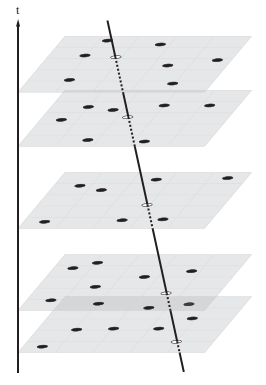
\includegraphics[width=6cm]{images/uniform_linear_motion}
		  \caption{Uniform linear motion throughout successive images. Image downloaded from \citep{oda}.}
	  \label{fig:u_l_m}
	\end{figure}